\chapter{Singular Value Decomposition}

Given a complex matrix $ A $ having \textit{m} rows and $ n $ columns, the matrix product $ U\Sigma V^T $ is a singular value
decomposition for a given matrix $ A $ if
\begin{itemize}
\item $ U $ and $ V $, respectively, have orthonormal columns. 
\item $\Sigma$  has nonnegative elements on its principal diagonal and zeros elsewhere.
\item $ A=U\Sigma V^T $
\end{itemize}
One application of the SVD is data compression. Consider some matrix $ A $ with rank five hundred; that is, the columns of this matrix span a 500-dimensional space. Encoding this matrix on a computer is going to take quite a lot of memory! We might be interested in approximating this matrix with one of lower rank. How close can we get to this matrix if we only approximate it as a matrix with rank one hundred, so that we only have to store a hundred columns?\\
It turns out that you can prove that taking the $ n $ largest singular values $ A $, replacing the rest with zero (to form $ \Sigma $), and recomputing $U\Sigma V^T $ gives you the provably best $ n $-rank approximation to the matrix. \cite{svdintro}


It means that we can take a list of $ n $ unique vectors, and approximate them as a linear combination of $ k $ unique vectors.\cite{svdquora}


  
    \begin{figure}[h!]
    	\centering
    	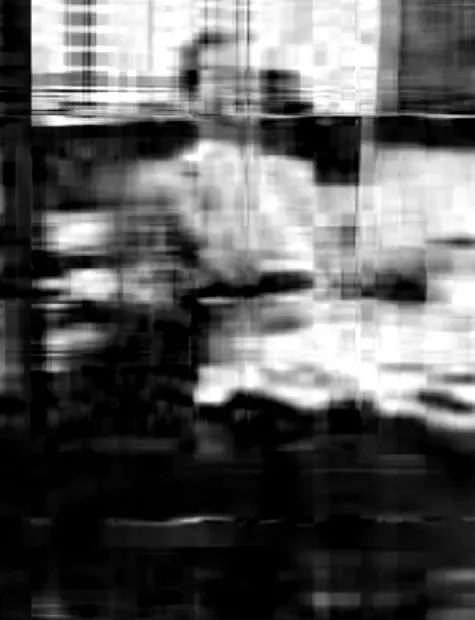
\includegraphics[width=0.75\textwidth]{imm/svd/10vectors.png} 	\caption{Image made of k=10 unique row vectors
    	} 
    	\label{k10}
    \end{figure}
    
      \begin{figure}[h!]
      	\centering
      	
\includegraphics[width=0.75\textwidth]{imm/svd/50vettori.png} 	\caption{Image made of k=50 unique row vectors
      	} 
      	\label{k50}
      \end{figure}
      
        \begin{figure}[h!]
        	\centering
        	
\includegraphics[width=0.75\textwidth]{imm/svd/400vettori.png} 	\caption{Image made of 400 unique row vectors
        	} 
        	\label{k400}
        \end{figure}
      \clearpage
\section{Example of a SVD computation}

For simplicity, we compute the SVD of a 2x2 matrix C:
\begin{center}
	$ 
	C=\begin{bmatrix}
	5 &   5 \\
-1  &  7 \\
	\end{bmatrix}$
\end{center}
and we want to write it as $ C=U\Sigma V^{T} $.\\
We have to take into account these 2 equations:
\begin{itemize}
	\item $ C^T C = V\Sigma^T\Sigma V^T$
	\item $CV=U\Sigma$
\end{itemize}
We first use the first equation  $ C^T C = V\Sigma^T\Sigma V^T$, and find the eigenvalues and the eigenvectors of $C^T C $.
The eigenvalues will be the entries of the diagonal entries of $ \Sigma^T\Sigma $, while the eigenvectors will be the entries of $ V $.\\
Let's compute $ C^T \cdot C $\\
\begin{center}
	$ C^T \cdot C =\begin{bmatrix}
5 &   -1 \\
5  &  7 \\
\end{bmatrix}\begin{bmatrix}
5 &   5 \\
-1  &  7 \\
\end{bmatrix}=\begin{bmatrix}
26 &   18 \\
18  &  74 \\
\end{bmatrix}$\\
\end{center}
Now we can find the eigenvalues of the matrix $ C^T \cdot C $.\\
We know that an eigenvalue of $ C^T \cdot C $, is a solution of the polynomial equation $det( C^T \cdot C-\lambda I)=0 $, where $ I $ is the identity matrix.\\
\begin{center}
	$det( C^T \cdot C-\lambda I)=det\begin{pmatrix}\begin{bmatrix}
26 &   18 \\
18  &  74 \\
\end{bmatrix}-\lambda\begin{bmatrix}
1 &   0 \\
0  &  1 \\
\end{bmatrix}\end{pmatrix}=$
\end{center}\begin{center}

=$det\begin{bmatrix}
26-\lambda &   18 \\
18  &  74-\lambda \\
\end{bmatrix}=(26-\lambda)(74-\lambda)-18\cdot 18=$
\end{center}

\begin{center}
	$= \lambda^2-100\lambda+1600 $
\end{center}
Since $ \lambda^2-100\lambda+1600 $ is a second degree equation, we can solve it using the general formula \begin{center}
	$ a\lambda^2+b\lambda+c $\end{center}

\begin{center}
		$\lambda=\dfrac{-b\pm\sqrt{b^2-4ac}}{2a}$

\end{center}
\begin{center}
	$\lambda=\dfrac{-100\pm\sqrt{100^2-4\cdot1600}}{2}$
	
\end{center}
which will provide the two solutions $ \lambda_1=20 $ and $\lambda_2=80$.\\
Now we want to find the eigenvector associated to the eigenvalue $ \lambda_1=20 $. We know that this eigenvector $ \textbf{v} $ solve the equation $ (C^T \cdot C-\lambda I)\textbf{v}=0 $ \\
\begin{center}
	$  (C^T \cdot C-\lambda_1 I)v_1= (C^T \cdot C-20 I) v_1= \begin{bmatrix}
	6 &   18 \\
	18  &  54\\
	\end{bmatrix}\begin{bmatrix}v_{1,1}\\v_{1,2}\end{bmatrix}=0 $
\end{center}
We can see it as an equations system
\begin{center}
	
$ \begin{cases} 6\cdot v_{1,1}+18 \cdot v_{1,2}=0 \\
   18\cdot v_{1,1}+54 \cdot v_{1,2}=0 \end{cases} $
\end{center}
and have $ v_{1,1}=-3 $,\quad $ v_{1,2}=1 $,\quad therefore $v_1=\begin{bmatrix}
-3\\
1
\end{bmatrix}$.\\
If we want the matrix $ V $ to be othonormal, then each vector of the matrix $ V $ has to be a unit vector (i.e. have lenght 1). To make it possible, we divide each entries of the vector by the lenght of the vector.
The lenght of $v_1$ is:
\begin{center}
	$ |v_1| = \sqrt{v_{1,1}^2+v_{1,2}^2}=\sqrt{(-3)^2+1^2}=\sqrt{10}$
\end{center}
\begin{center}
	$ v_1=\begin{bmatrix}
	\frac{-3}{\sqrt{10}}\\
	\frac{1}{\sqrt{10}}
	\end{bmatrix} $
\end{center}

Now we can do the same steps for the second eingenvector
\begin{center}
		$  (C^T \cdot C-\lambda_2 I)v_2=( C^T \cdot C-80 I) v_2= \begin{bmatrix}
		-54 &   18 \\
		18  &  -6\\
	\end{bmatrix}\begin{bmatrix}v_{2,1}\\v_{2,2}\end{bmatrix}=0  $
\end{center}
\begin{center}
	
	$ \begin{cases} -54\cdot v_{2,1}+18 \cdot v_{2,2}=0 \\
	18\cdot v_{2,1} -6 \cdot v_{2,2}=0 \end{cases} $
\end{center}
\begin{center}
	$  v_2=\begin{bmatrix}
	1\\
	3
	\end{bmatrix}$ $ \Longrightarrow $ orthonormal$ \Longrightarrow $ $v_2=\begin{bmatrix}
	\frac{1}{\sqrt{10}}\\
	\frac{3}{\sqrt{10}}
	\end{bmatrix}  $
\end{center}
Now we can write the matrix $ V $
\begin{center}
	$ V=\begin{bmatrix}
	v_1 & v_2
	\end{bmatrix}=\begin{bmatrix}
	\frac{-3}{\sqrt{10}} & \frac{1}{\sqrt{10}}\\
	\frac{1}{\sqrt{10}} &	\frac{3}{\sqrt{10}}
	\end{bmatrix} $
\end{center}
and the matrix $ \Sigma $. We know that  $ \Sigma $ is a diagonal matrix, so its transpose matrix is $ \Sigma^T= \Sigma  $, and doing $\Sigma^T \Sigma$ is the same thing of doing the square of each diagonal entries of $\Sigma$.
As said before at the beginning, the eigenvalues are the entries of $\Sigma^T \Sigma$, so to find the matrix $\Sigma$ we just need to make the square root of the eigenvalues and put them in diagonal.
\begin{center}
	$ \Sigma=\begin{bmatrix}
	\sqrt{\lambda_1} & 0\\
	0 & \sqrt{\lambda_2}
	\end{bmatrix}=\begin{bmatrix}
		\sqrt{20} & 0\\
		0 & \sqrt{80}
	\end{bmatrix}=\begin{bmatrix}
	2\sqrt{5} & 0\\
	0 & 4\sqrt{5}
	\end{bmatrix} $
\end{center}
Now we need to find the last part of the SVD, which is the matrix $ U $. To find it we use the second property listed at the beginning of this section\\
\begin{itemize}
	\item $CV=U\Sigma$
\end{itemize}
\begin{center}
	$ CV=\begin{bmatrix}
		5 &   5 \\
		-1  &  7 \\
	\end{bmatrix}\begin{bmatrix}
	\frac{-3}{\sqrt{10}} & \frac{1}{\sqrt{10}}\\
	\frac{1}{\sqrt{10}} &	\frac{3}{\sqrt{10}}
	\end{bmatrix}=\begin{bmatrix}
	-\sqrt{10} & 2\sqrt{10}\\
	\sqrt{10} &	2\sqrt{10}
	\end{bmatrix}=U\Sigma $
\end{center}
To find $U$, we have to decompose $\begin{bmatrix}
-\sqrt{10} & 2\sqrt{10}\\
\sqrt{10} &	2\sqrt{10}
\end{bmatrix}$ as the product of $U$ and $\Sigma$

\begin{center}
	 $\begin{bmatrix}
	 -\sqrt{10} & 2\sqrt{10}\\
	 \sqrt{10} &	2\sqrt{10}
	 \end{bmatrix}= \begin{bmatrix}
	 	u_{1,1} & u_{1,2} \\
	 	u_{2,1} & u_{2,2}
	 \end{bmatrix}\begin{bmatrix}
	 2\sqrt{5} & 0\\
	 0 & 4\sqrt{5}
	 \end{bmatrix}$\\
\end{center}
If we split the matrix, we obtain
\begin{center}
	
	$ -\sqrt{10}=	u_{1,1} \cdot 2\sqrt{5} + u_{1,2} \cdot 0$\quad $ \Longrightarrow $ \quad $ 	u_{1,1}=-\frac{1}{\sqrt{2}} $\\
	
	$2\sqrt{10}=	u_{1,1} \cdot 0 + u_{1,2} \cdot 4\sqrt{5}$\quad $ \Longrightarrow $ \quad $ 	u_{1,2}=\frac{1}{\sqrt{2}} $\\
	
	$ \sqrt{10}=	u_{2,1} \cdot 2\sqrt{5} + u_{2,2} \cdot 0$\quad $ \Longrightarrow $ \quad $ 	u_{2,1}=\frac{1}{\sqrt{2}} $\\
	
	$2\sqrt{10}=	u_{2,1} \cdot 0 + u_{2,2} \cdot 4\sqrt{5}$\quad $ \Longrightarrow $ \quad $ 	u_{2,2}=\frac{1}{\sqrt{2}} $\\
\end{center}

Then finally 

\begin{center}
	$ U=\begin{bmatrix}
	\frac{-1}{\sqrt{2}} & \frac{1}{\sqrt{2}}\\
	\frac{1}{\sqrt{2}} & \frac{1}{\sqrt{2}}
	\end{bmatrix} $
\end{center}
\section{Difficulties for the SVD in ASIC}
As you can see in the example above, the SVD is a complex algorithm. I had some problems in designing it in ASIC especially for a generic matrix $ n$x$n $.
In order we have
\begin{itemize}
	\item \textbf{Determinant}, find the determinant requires times and memory. Greater the dimension of the matrix, harder the computation of the determinant.
	\item \textbf{Eigenvalues} assuming we have find the Characteristic polynomial of the matrix, we will have a polynomial equation of degree $ n $, and we have to find $ n $ solutions of this polynomial in hardware.
	\item \textbf{Eigenvectors} assuming we have all the $ n $ eigenvalues, for each of the we have to solve a system of $n$ equations with $n$ variables. In total there will be $n^2$ equations to be solved.
\end{itemize}
